\usetikzlibrary{shapes.geometric}
\usetikzlibrary{angles}
\definecolor{myblue}{rgb}{0.067,0.529,0.871}
\definecolor{mypurple}{rgb}{0.859,0.071,0.525}
\definecolor{myred}{rgb}{1.0, 0.13, 0.32}
\definecolor{mygreen}{rgb}{0.01, 0.75, 0.24}
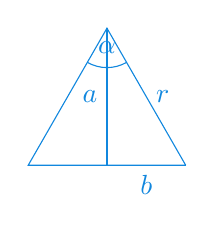
\begin{tikzpicture}[draw=myblue, text=myblue]
\coordinate (A) at (-1,-1.74);
\coordinate (B) at (0,0);
\coordinate (C) at (1,-1.74);
\draw pic[draw, angle radius=0.5cm]{angle=A--B--C};
\node at (0,-0.25) {$\alpha$};
\draw (C) -- (A) -- (B) -- (C) node[right, midway] {$r$};
\draw (B) -- (0,-1.74) node[left, midway] {$a$};
\draw (0, -1.74) -- (C) node[below, midway] {$b$}; 
\end{tikzpicture}
